\section{Dashboard}
\label{sec:Dashboard}
It is extremely important for our developers and project managers to have a
quick overview on the status of the nightly builds, and this view should be
tunable so that each user can see only the informations relevant to her.

For the prototype of the new nightly builds system we considered two
possibilities: CDash and the summary web page of the old system.

\subsection{CDash}
\label{Dashboard:CDash}
CDash is the dashboard solution developed for integration with the CTest tool
bundled with CMake.

CTest can be used to build and test projects based on CMake as well as on custom
tools.  Of course, CMake projects are easier to handle than the others, but it
has not been too difficult to develop a working script for CMT-based projects,
as described in \ref{sec:CoreTools:Build}.

To try to reproduce a structure similar to the one we need, we declared each
slot as a project in CDash and all the software projects in the slot as
sub-projects\cite{CMakeBook,CDashSubprojects} (using the combination of name and
version as CDash sub-project names).  The platform id string translates to the
\emph{build name} and we use the build slave hostname as \emph{site}.  In order
to display enough informations, the CDash projects representing the slots must
be configured to be public and display \emph{labels} (special meta-data fields
used to identify the builds of the sub-projects).

With this configuration, the first page we get when connecting to our CDash
instance (currently \urlLink{https://lbtestbuild.cern.ch/CDash}) contains the
list of the declared slots (if a slot is not declared to CDash, it will not
appear even if it has been built and the result pushed to the server) with a
description, but without any information on the status of the build
(Figure~\ref{fig:cdash-home}).

\begin{figure}
  \begin{center}
    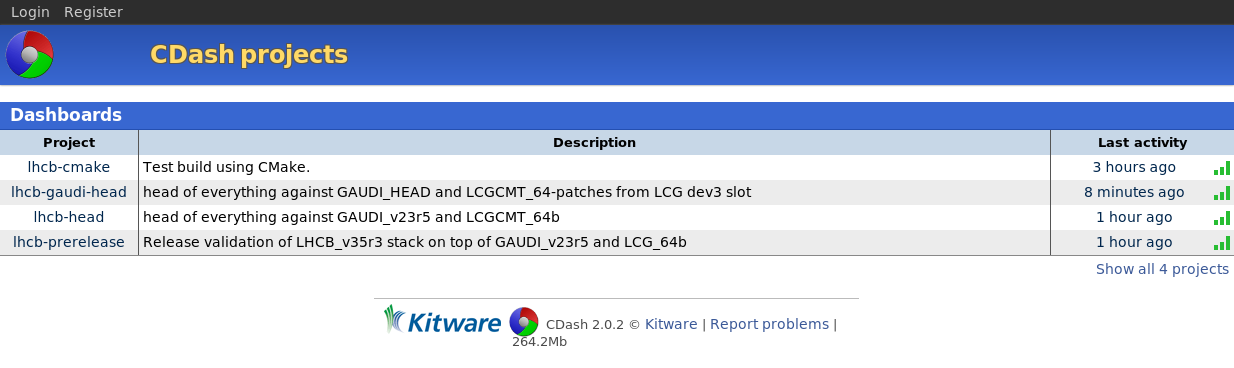
\includegraphics[width=15cm]{cdash-1}
  \end{center}
  \caption{CDash: Initial page with the list of slots.}
  \label{fig:cdash-home}
\end{figure}

Clicking on one of the slots, we can access the overview page for that slot,
where the number of successful or problematic builds is reported
(Figure~\ref{fig:cdash-slot}).

\begin{figure}
  \begin{center}
    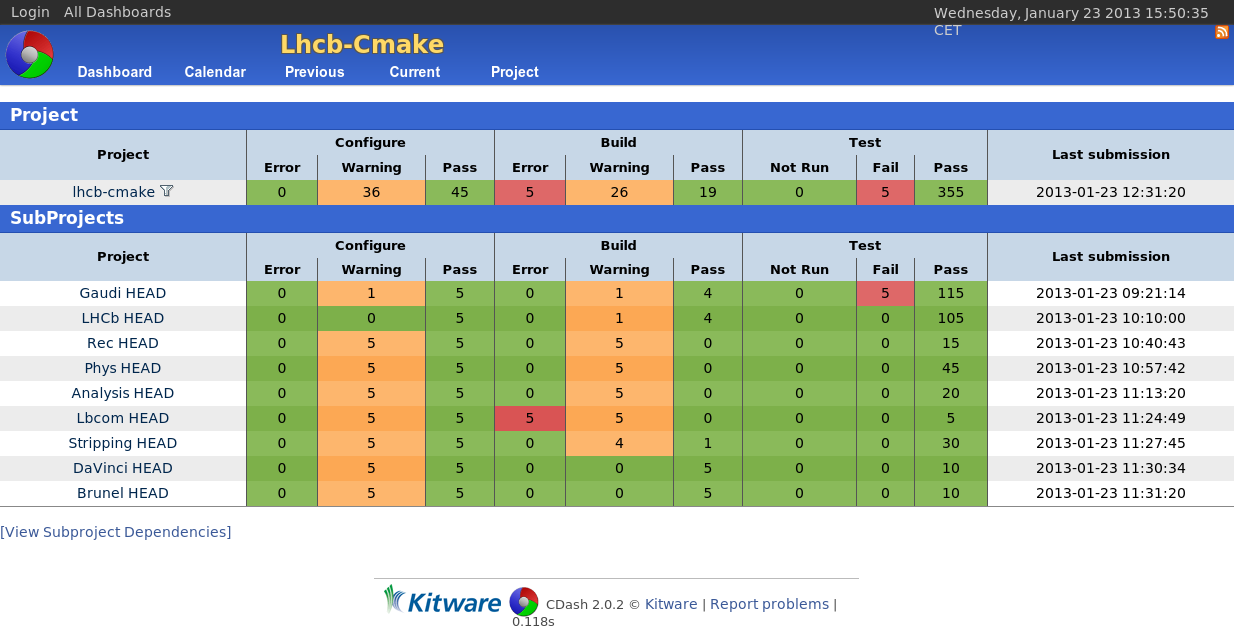
\includegraphics[width=15cm]{cdash-2}
  \end{center}
  \caption{CDash: Overview of one slot.}
  \label{fig:cdash-slot}
\end{figure}

We can go deeper and see the details of the builds of project in the slot
(Figure~\ref{fig:cdash-project}) or a summary for a platform
(Figure~\ref{fig:cdash-platform}).

\begin{figure}
  \begin{center}
    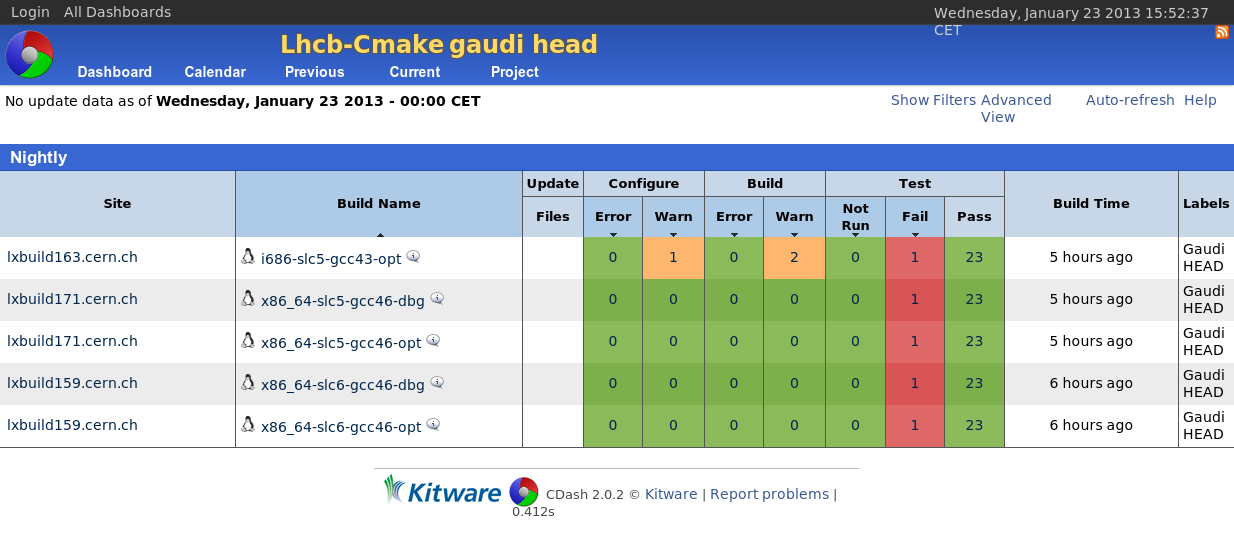
\includegraphics[width=15cm]{cdash-3}
  \end{center}
  \caption{CDash: Detailed view of a project in one slot.}
  \label{fig:cdash-project}
\end{figure}

\begin{figure}
  \begin{center}
    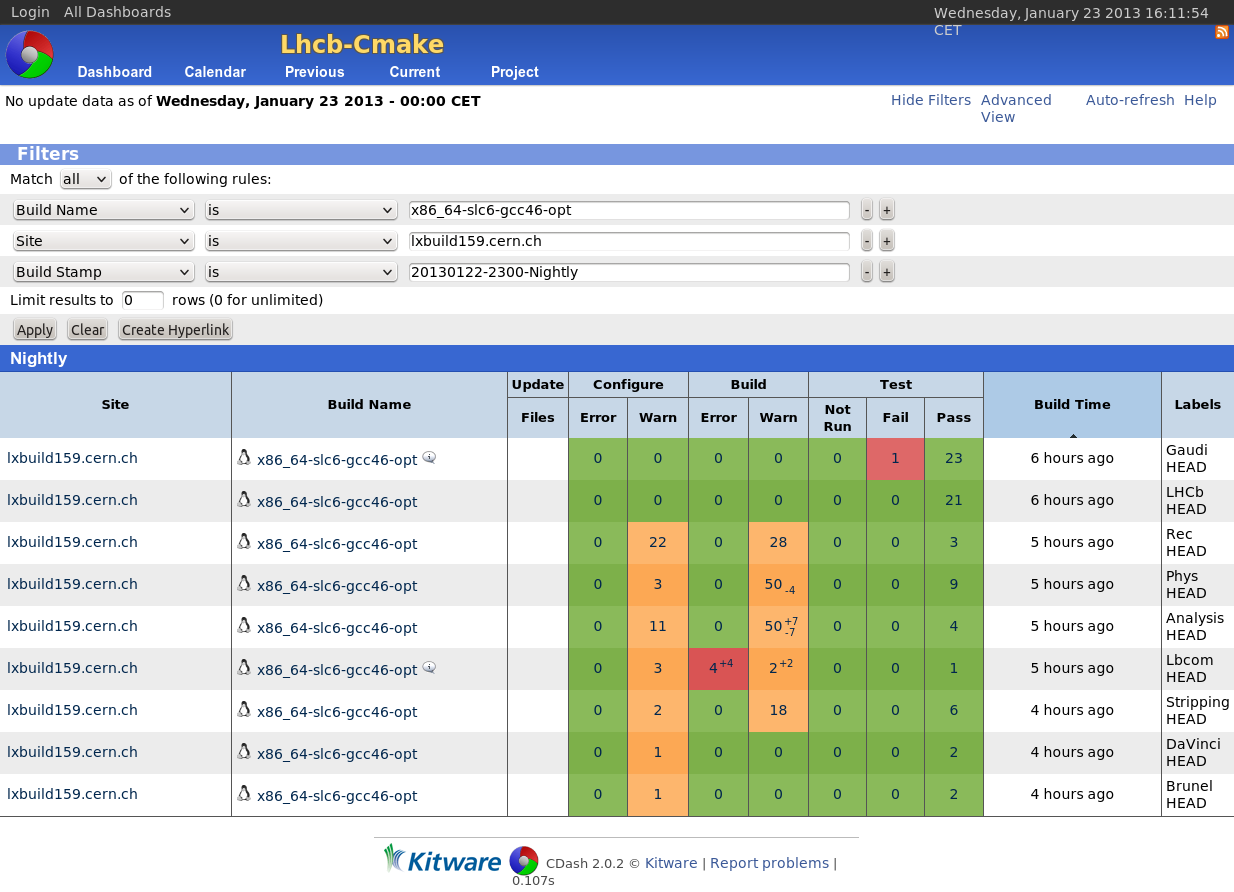
\includegraphics[width=15cm]{cdash-4}
  \end{center}
  \caption{CDash: Overview of a platform in one slot.}
  \label{fig:cdash-platform}
\end{figure}

It must be noted that the tests we run in our nightly builds use
QMTest\cite{QMTestPaper} (as mentioned in \ref{sec:CoreTools:Build}).  When using
CTest, we start a collection of QMTest tests as a single CTest test, so the
numbers in the CDash views (Figure~\ref{fig:cdash-project}) are not correct,
while, when we use CMT, we cannot even publish the results of the tests to
CDash, so those fields are empty.  The plan is to extend the output format of
QMTest to produce result files in a format understood by CDash, so that we can
publish the correct informations.  In the long term we will also replace QMTest
with CTest, but the extension of the output format is the only possibility in
the short term.

The informations stored in the CDash database are enough for out purposes (apart
from the results of the tests), but the layout is not optimal for our purposes.
Since we build the same version of a project in several contexts, it is useful
to see all its builds across the slots, but this is impossible with CDash.
Moreover, the view in Figure~\ref{fig:cdash-platform} puts the accent on the
wrong information (the site), while we give more importance to the project
(label).  We also observed some annoying bugs which might be fixed in a future
version (the latest release is one year old).  Anyway, since CDash is open
source, we could extend it, more or less easily, to extract from the database
the details we need and display them the way we like.

\subsection{Old Summary Web Page}
\label{sec:Dashboard:Old}
The summary web page of the old system was designed to convey all the needed
informations in a single view (Figure~\ref{fig:old-summary}), so its layout and
infrastructure could be reuses.  To evaluate the feasibility of this approach,
we produce with the new system partial summary files for the build and tests
that are compatible with the expectations of the old system.

\begin{figure}
  \begin{center}
    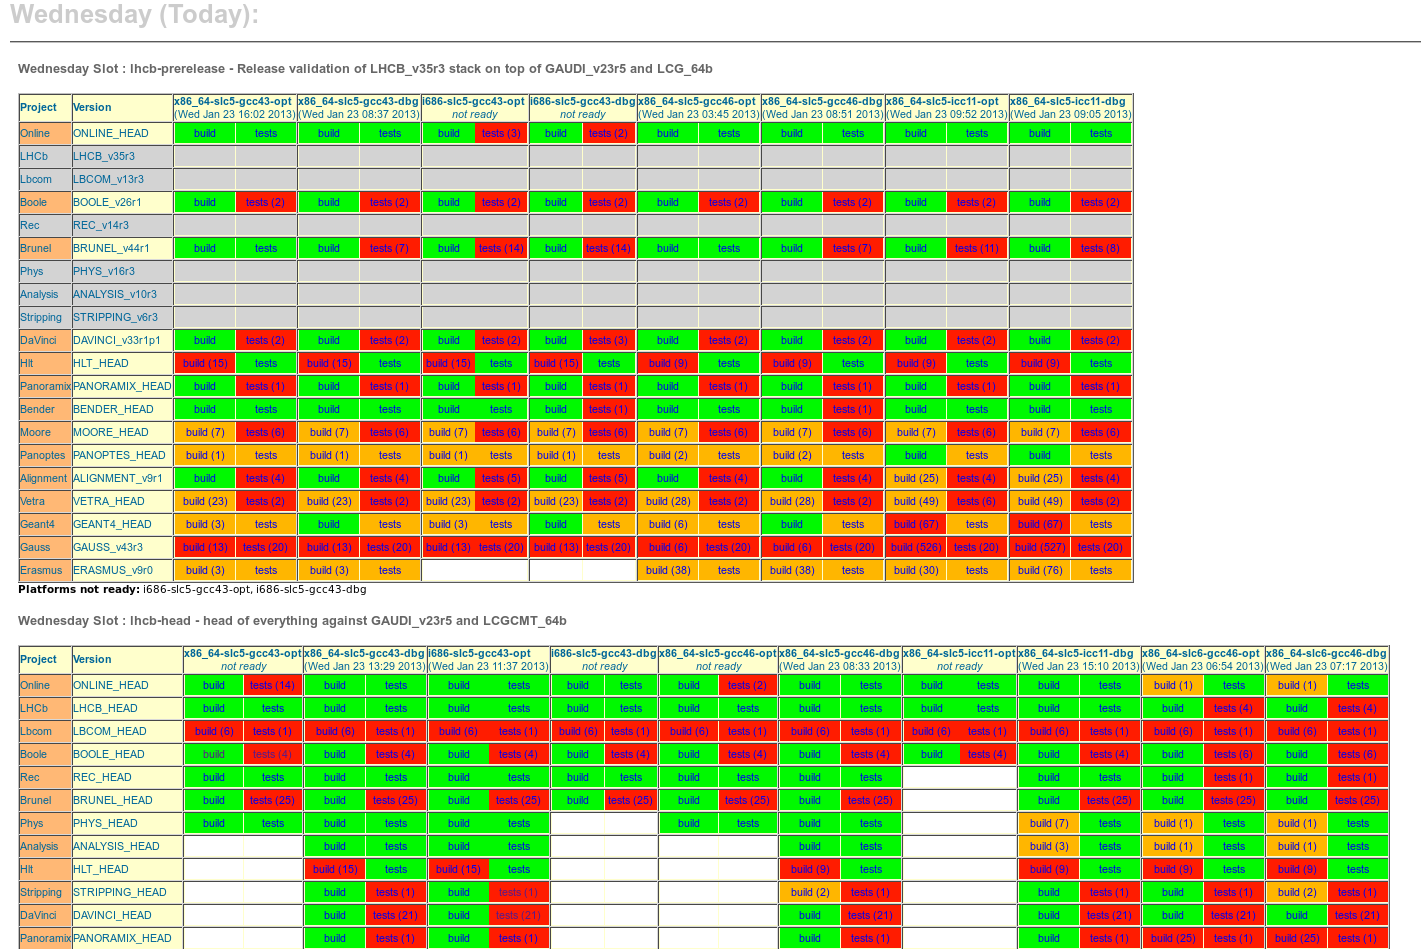
\includegraphics[width=15cm]{old-summary}
  \end{center}
  \caption{Old Summary Web Page: Part of the summary tables.}
  \label{fig:old-summary}
\end{figure}

Although possible, there are several downsides in this approach.

The parsing of the build and test log files is partially integrated in the build
step of the old system and partially in the regular job that generates the full
version of the summary page.  To produce the data required by the regular job we
need to rewrite from scratch the parsing code to extract it from the old build
step.

The technology used for the summary page is obsolete: a static HTML file
produced by a job run every 15 minutes, which is then filtered by a CGI script.
A more modern approach would involve dynamic content (currently achieved by
forcing a reload of the full page) and an independent exchange format, such as
XML, with the possibility of a layout usable on small screens (smart phones).

The amount of work required to reproduce completely the old summary files will
be probably spent better in the extension of CDash or Jenkins, or in the
development of a completely new dashboard.
